%\documentclass[handout]{beamer}
\documentclass[10pt]{beamer}
%for(int i=0; i<n; i++){\documentclass[10pt,handout]{beamer}
\usepackage[spanish]{babel}
% % \usepackage[backend=biber, style=authoryear-icomp]{biblatex}
\resetcounteronoverlays{exx}
\usepackage{mdframed}
\usepackage{tikz}
\usepackage{blindtext}
\usepackage{tipa}
% \usepackage{cgloss4e}
% \usepackage{gb4e}
% \usepackage{qtree}
\usepackage{cancel}
\usepackage{wrapfig}
\usepackage{soul}
\usepackage{enumerate}
\usepackage{longtable}
\graphicspath{ {./figures/} } % declaramos donde estan las imagenes
\usepackage[labelformat=simple]{subcaption} % para varias imagenes juntas
\renewcommand\thesubfigure{(\alph{subfigure})}
\usepackage[utf8]{inputenc}
\usepackage{amsmath}
\usepackage{amsfonts} % simbolos como el I de matriz identidad
\usepackage{bm}
\usepackage{graphicx} % paquete para ver imagenes
\usepackage{setspace}
\usepackage[T1]{fontenc}
\usepackage{parskip}
\usepackage{color}
\usepackage{framed}

\usetheme{Copenhagen}
\definecolor{frenchblue}{rgb}{0.0, 0.45, 0.73} % ESTE!!!!

\setbeamercolor{block body}{bg=frenchblue!50}
\setbeamercolor*{structure}{fg=frenchblue,bg=blue}
\setbeamercolor{normal text}{fg=black}
\setbeamercolor{frametitle}{bg=black}
\setbeamertemplate{frametitle}[default][center]
\setlength{\parskip}{12pt}
\useoutertheme{infolines} % me comia mucho espacio de la otra fgorma
\makeatother
\setbeamertemplate{footline}
{
  \leavevmode%
  \hbox{%
  \begin{beamercolorbox}[wd=.3\paperwidth,ht=2.25ex,dp=1ex,center]{author in head/foot}%
    \usebeamerfont{author in head/foot}\insertshortauthor
  \end{beamercolorbox}%
  \begin{beamercolorbox}[wd=.6\paperwidth,ht=2.25ex,dp=1ex,center]{title in head/foot}%
    \usebeamerfont{title in head/foot}\insertshorttitle
  \end{beamercolorbox}%
  \begin{beamercolorbox}[wd=.1\paperwidth,ht=2.25ex,dp=1ex,center]{date in head/foot}%
    \insertframenumber{} / \inserttotalframenumber\hspace*{1ex}
  \end{beamercolorbox}}%
  \vskip0pt%
}
\makeatletter
\setbeamertemplate{navigation symbols}{}
%\setbeameroption{show notes}
\setbeameroption{hide notes}
\renewcommand{\CancelColor}{\color{red}}

\usepackage{hyperref}

\title[Flip-Flop JK]{Organizaci\'on del Computador I: Flip-Flop JK}
\author[Matias Mazzanti]{Matias Mazzanti}


\institute{DC-UBA}
\date{09 de Agosto de 2022}

\titlegraphic{
\includegraphics[,height=2cm,keepaspectratio]{../../logo.pdf}     }
%\logo{
\includegraphics[height=2.5cm]{logo.PDF}}

\begin{document}

\begin{frame}

\maketitle

\end{frame}


\section{Presentaci\'on}
\begin{frame}
\frametitle{Introducción}
\begin{mdframed}[backgroundcolor=frenchblue!20]
  Tema del día: Flip-Flops JK
\end{mdframed}
\pause

\begin{itemize}
  \item Repaso.
  \item Definición.
  %\item Motivación.
  \item Ejercicio.
  \item Solución.
  \item Conclusiones.
\end{itemize}

\end{frame}
\begin{frame}
\frametitle{Repaso}
En donde estábamos?

\pause
Circuitos \textbf{Combinacionales}: La salida  esta determinada únicamente por la entrada
del circuito.

\pause
Circuitos \textbf{Secuenciales}: La salida esta determinada por la entrada y por el \textbf{estado}
del circuito.
\begin{columns}
    \column{0.5\textwidth}

Estos los podemos pensar como un bloque combinacional y un bloque con memoria.

\pause
Donde E es la entrada S es la salida y  Q$_n$ el estado de la memoria en tiempo $n$.
    \column{0.5\textwidth}
        \begin{figure}[h!]
    \centering
    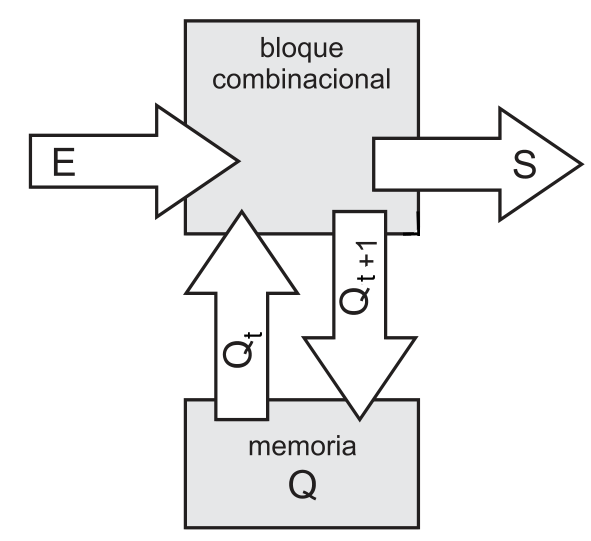
\includegraphics[scale=0.2]{secuencial.png}
\end{figure}
\end{columns}

\end{frame}

\begin{frame}
\frametitle{Repaso}

\begin{columns}
      \column{0.5\textwidth}
        \begin{figure}[h!]
            \centering
            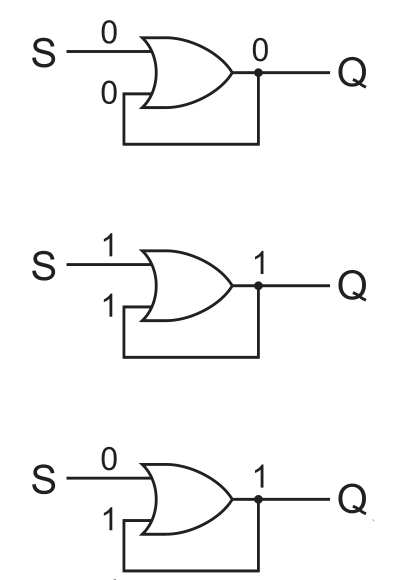
\includegraphics[scale=0.3]{unbit.png}
        \end{figure}
    \column{0.5\textwidth}
        Vimos que al intentar almacenar un bit de la forma trivial: un OR o AND.

        El circuito se \textbf{traba}.

\pause
\vspace{1cm}
Luego de almacenar un valor, no puedo cambiarlo.
\vspace{1cm}
\pause

Ademas me interesa tener control sobre cuando podemos cambiar el valor almacenado!
\pause $\to$
Se\~nal de clock!

\end{columns}
\end{frame}

\begin{frame}
\frametitle{Repaso}
\begin{mdframed}[backgroundcolor=frenchblue!20]
  El Flip-Flop resuelve este problema con m\'as de un componente y con retroalimentaci\'on.
\end{mdframed}
\vspace{0.2cm}
\begin{columns}
\pause
      \column{0.5\textwidth}
        Flip-Flops RS: Reset and Set

         \begin{figure}[h!]
             \centering
             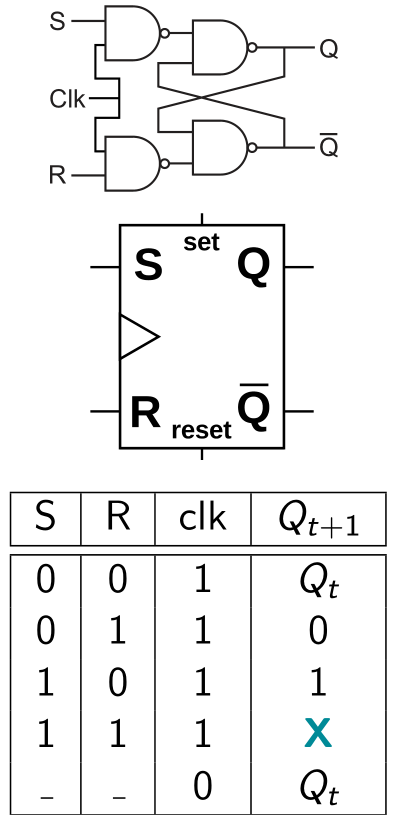
\includegraphics[scale=0.18]{flipRS.png}
         \end{figure}
    \column{0.5\textwidth}
\pause
        Flip-Flops D: Delay

\begin{figure}[h!]
    \centering
    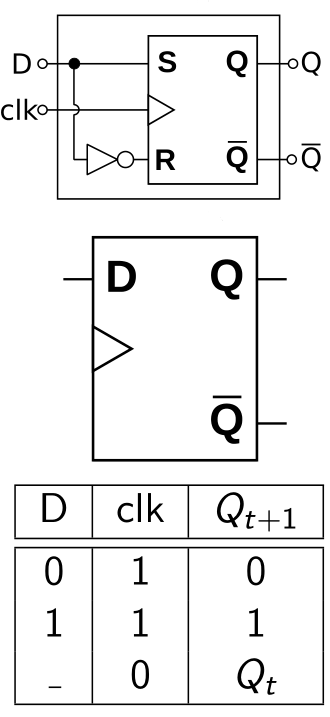
\includegraphics[scale=0.18]{flipD.png}
\end{figure}


\end{columns}

\end{frame}

\begin{frame}
\frametitle{Flip-Flop JK}
\only<1,2,3>{Flip-Flop JK resuelve el problema del input R=1 y S=1 del RS.

\pause
Ademas aprovecha el delay para generar cambios solo en los flancos de la se\~nal de clock.

Que pasa cuando en el JK ambas entradas son 1?
\pause
\begin{figure}[h!]
    \centering
    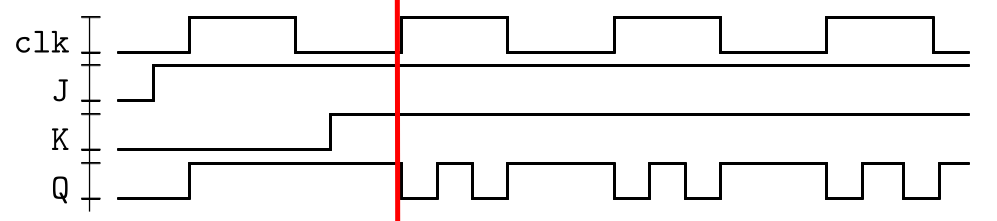
\includegraphics[scale=0.2]{delay2.png}
\end{figure}
Esto nos sirve?
}
\only<4>{
  Flip-Flop JK resuelve el problema del input R=1 y S=1 del RS.

Ademas aprovecha el delay para generar cambios solo en los flancos de la se\~nal de clock.

Que pasa cuando en el JK ambas entradas son 1?\begin{figure}[h!]
    \centering
    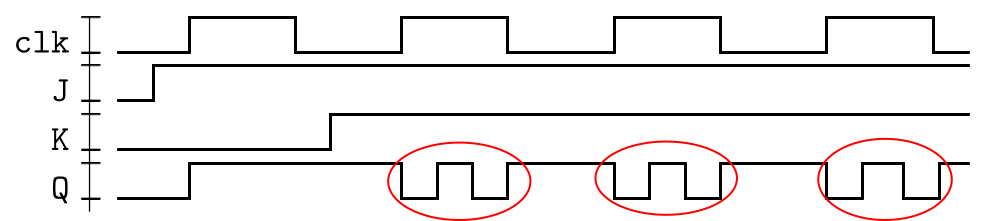
\includegraphics[scale=0.2]{delay3.png}
\end{figure}
Esto nos sirve? Se mueve dentro de un mismo pulso de clock...
}

\end{frame}

\begin{frame}
\frametitle{Flip-Flop JK}

Solución: \textbf{detector de pulsos}. Miro solo los flancos.

Circuito AND, único input duplicado,  negando una de las entradas.
\begin{figure}[h!]
    \centering
    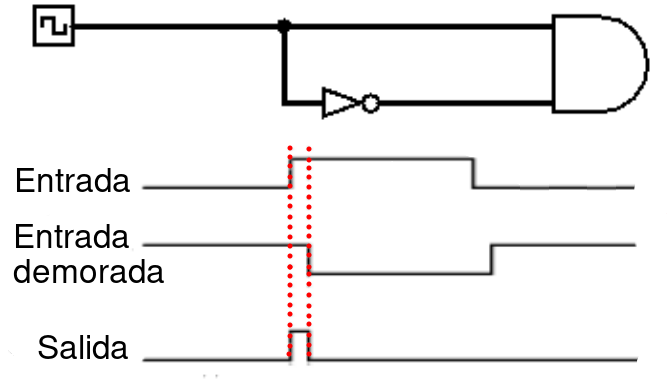
\includegraphics[scale=0.2]{delay.png}
\end{figure}

\pause

\begin{figure}[h!]
    \centering
    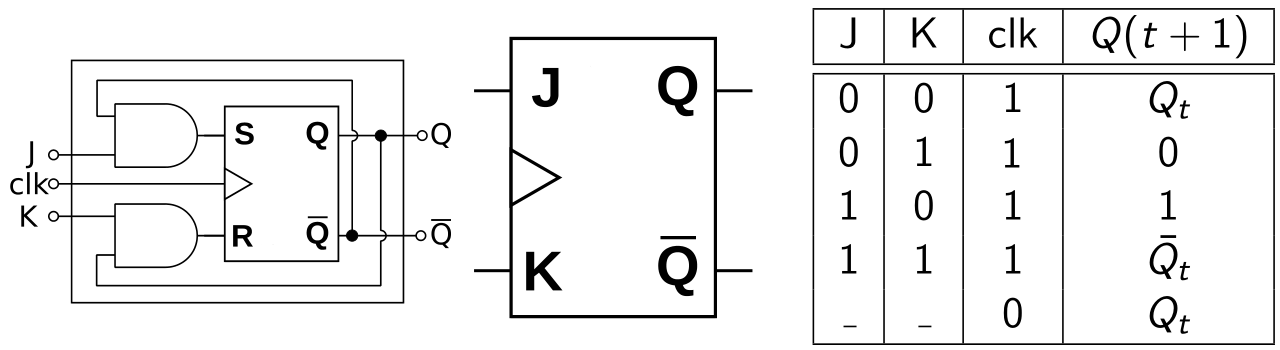
\includegraphics[scale=0.2]{flipJK.png}
\end{figure}


\end{frame}
%\begin{frame}
%\frametitle{Motivación}
%
%Al poder dominar el almacenamiento de un bit de forma controlada, permite poder construir
%cualquier tipo de almacenamiento.
%
%\pause
%No necesariamente las memorias modernas utilizan esta tecnología.
%
%\pause
%Bloque fundamental de las  FPGA.
%
%\begin{figure}[h!]
%    \centering
%    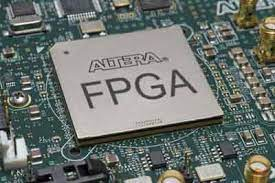
\includegraphics[scale=0.5]{fpga.jpeg}
%\end{figure}
%\end{frame}
%

\begin{frame}
\frametitle{Ejercicio}

Dado el siguiente circuito diga que función cumple.
Que modificación o agregado le haría para implementar un registro de dos bits
que siga los siguiente estados en donde cada cambio se produzca al apretar un pulsador.

\begin{columns}
    \column{0.5\textwidth}
        \begin{figure}[h!]
            \centering
          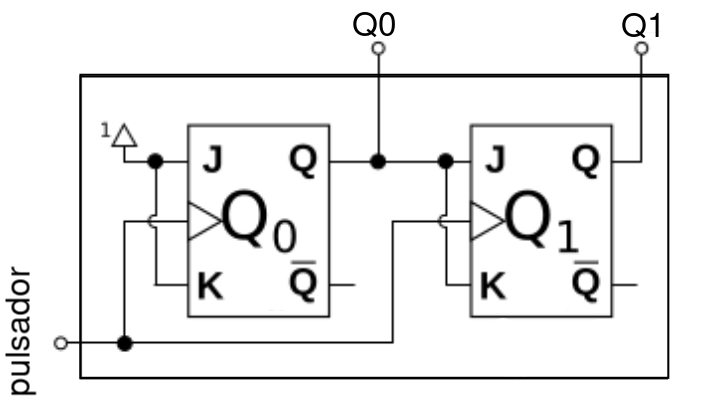
\includegraphics[scale=0.21]{circuito.png}
        \end{figure}
    \column{0.5\textwidth}
        \begin{figure}[h!]
          \centering
            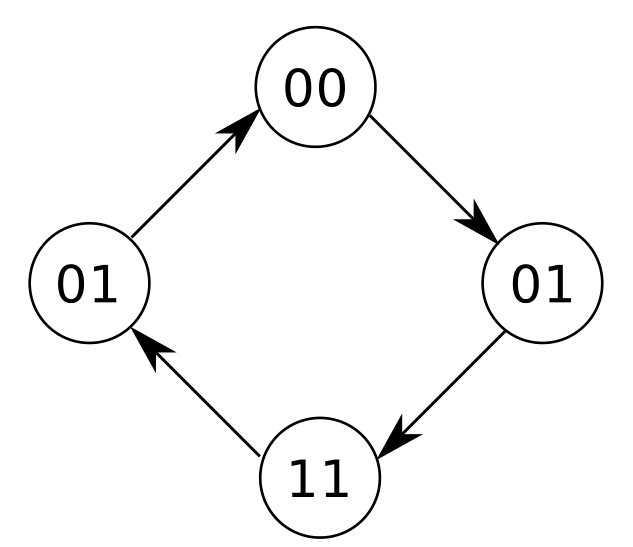
\includegraphics[scale=0.21]{ej1.png}
      \end{figure}
\end{columns}

\end{frame}

\begin{frame}
\frametitle{Solución parte a}
\only<1,2,3,4,5>{\begin{columns}
    \column{0.5\textwidth}
En principio.... ? Como arrancamos?
\pause

\begin{mdframed}[backgroundcolor=frenchblue!20]
  TABLAS DE VERDAD!
\end{mdframed}
\pause
\vspace{0.15cm}
REC: JK actualiza valor en J,K=1 y mantiene valor en J,K=0
\pause
    \column{0.5\textwidth}
\begin{figure}[h!]
    \centering
    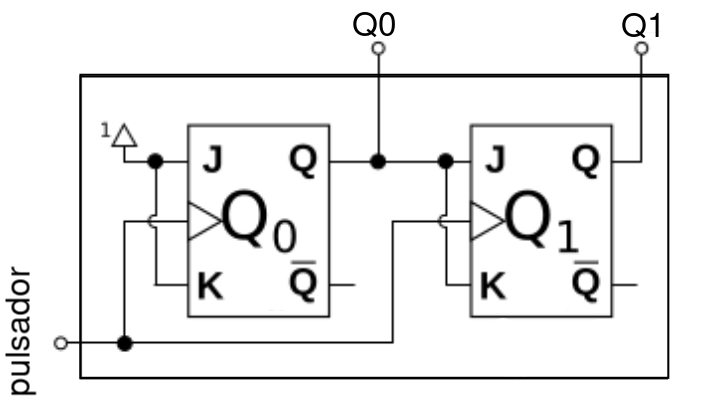
\includegraphics[scale=0.23]{circuito.png}
\end{figure}
\end{columns}
\pause
\begin{table}[h!]
\begin{tabular}{|c|c|c|c|c|}
\hline
Q$_1$(t) & Q$_0$(t) &  & Q$_1$(t+1) & Q$_0$(t+1) \\ \hline
0        & 0        &  &           &          \\ \hline
0        & 1        &  &           &           \\ \hline
1        & 0        &  &           &           \\ \hline
1        & 1        &  &           &           \\ \hline
\end{tabular}
\end{table}
El primer JK tiene todo 1 cambio, y el segundo todo 0 mantengo.}

\only<6>{\begin{columns}
    \column{0.5\textwidth}
En principio.... ? Como arrancamos?

\begin{mdframed}[backgroundcolor=frenchblue!20]
  TABLAS DE VERDAD!
\end{mdframed}
\vspace{0.15cm}
REC: JK actualiza valor en J,K=1 y mantiene valor en J,K=0
    \column{0.5\textwidth}
\begin{figure}[h!]
    \centering
    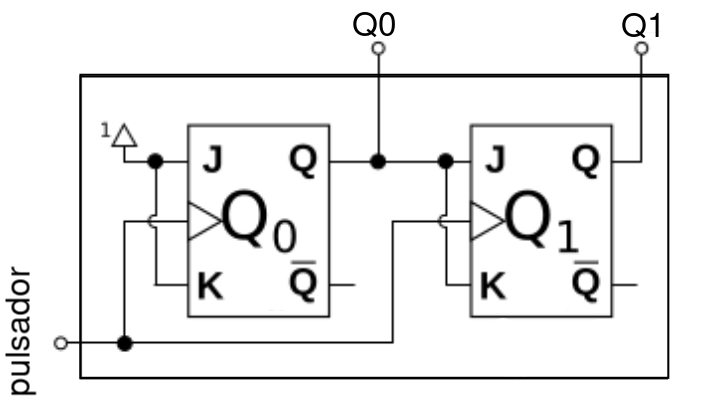
\includegraphics[scale=0.23]{circuito.png}
\end{figure}
\end{columns}
\begin{table}[h!]
\begin{tabular}{|c|c|c|c|c|}
\hline
Q$_1$(t) & Q$_0$(t) &  & Q$_1$(t+1) & Q$_0$(t+1) \\ \hline
0        & 0        &  & 0          & 1          \\ \hline
0        & 1        &  &           &           \\ \hline
1        & 0        &  &           &           \\ \hline
1        & 1        &  &           &           \\ \hline
\end{tabular}
\end{table}
El primer JK tiene todo 1 cambio, y el segundo todo 1 cambio.}
\only<7>{\begin{columns}
    \column{0.5\textwidth}
En principio.... ? Como arrancamos?

\begin{mdframed}[backgroundcolor=frenchblue!20]
  TABLAS DE VERDAD!
\end{mdframed}
\vspace{0.15cm}
REC: JK actualiza valor en J,K=1 y mantiene valor en J,K=0
    \column{0.5\textwidth}
\begin{figure}[h!]
    \centering
    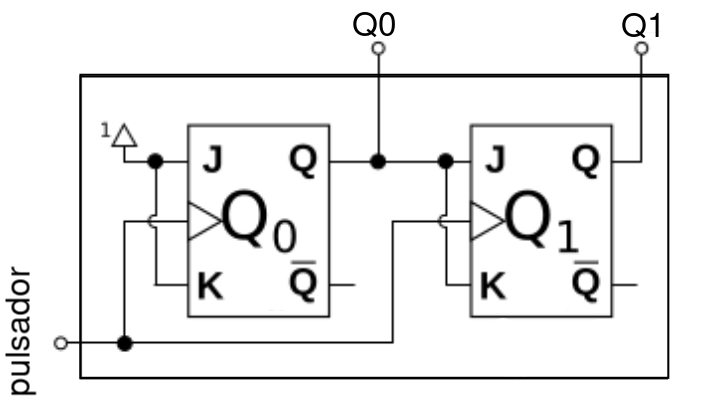
\includegraphics[scale=0.23]{circuito.png}
\end{figure}
\end{columns}
\begin{table}[h!]
\begin{tabular}{|c|c|c|c|c|}
\hline
Q$_1$(t) & Q$_0$(t) &  & Q$_1$(t+1) & Q$_0$(t+1) \\ \hline
0        & 0        &  & 0          & 1          \\ \hline
0        & 1        &  & 1          & 0          \\ \hline
1        & 0        &  &           &          \\ \hline
1        & 1        &  &           &           \\ \hline
\end{tabular}
\end{table}El primer JK tiene todo 1 cambio, y el segundo todo 0 mantengo.}

\only<8>{\begin{columns}
    \column{0.5\textwidth}
En principio.... ? Como arrancamos?

\begin{mdframed}[backgroundcolor=frenchblue!20]
  TABLAS DE VERDAD!
\end{mdframed}
\vspace{0.15cm}
REC: JK actualiza valor en J,K=1 y mantiene valor en J,K=0
    \column{0.5\textwidth}
\begin{figure}[h!]
    \centering
    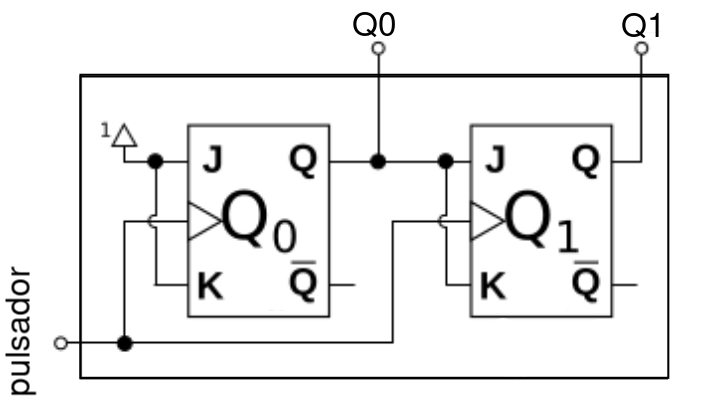
\includegraphics[scale=0.23]{circuito.png}
\end{figure}
\end{columns}
\begin{table}[h!]
\begin{tabular}{|c|c|c|c|c|}
\hline
Q$_1$(t) & Q$_0$(t) &  & Q$_1$(t+1) & Q$_0$(t+1) \\ \hline
0        & 0        &  & 0          & 1          \\ \hline
0        & 1        &  & 1          & 0          \\ \hline
1        & 0        &  & 1          & 1          \\ \hline
1        & 1        &  &           &           \\ \hline
\end{tabular}
\end{table}El primer JK tiene todo 1 cambio, y el segundo todo 1 cambio.}
\only<9>{\begin{columns}
    \column{0.5\textwidth}
En principio.... ? Como arrancamos?

\begin{mdframed}[backgroundcolor=frenchblue!20]
  TABLAS DE VERDAD!
\end{mdframed}
\vspace{0.15cm}
REC: JK actualiza valor en J,K=1 y mantiene valor en J,K=0
    \column{0.5\textwidth}
\begin{figure}[h!]
    \centering
    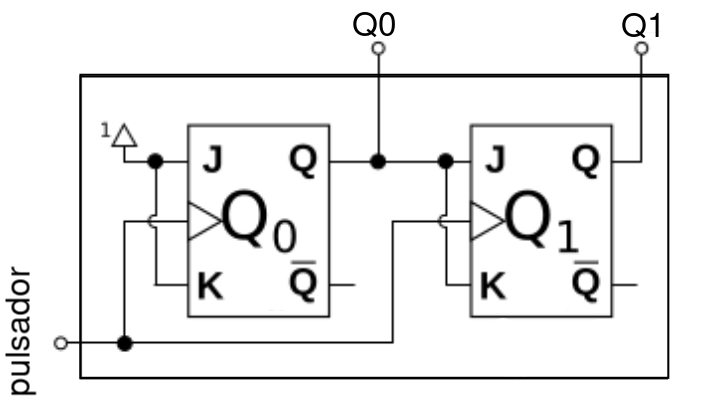
\includegraphics[scale=0.23]{circuito.png}
\end{figure}
\end{columns}
\begin{table}[h!]
\begin{tabular}{|c|c|c|c|c|}
\hline
Q$_1$(t) & Q$_0$(t) &  & Q$_1$(t+1) & Q$_0$(t+1) \\ \hline
0        & 0        &  & 0          & 1          \\ \hline
0        & 1        &  & 1          & 0          \\ \hline
1        & 0        &  & 1          & 1          \\ \hline
1        & 1        &  & 0          & 0          \\ \hline
\end{tabular}
\end{table}
Termine tabla de verdad, y ahora? A que se parece?
}
\only<10>{\begin{columns}
    \column{0.5\textwidth}
En principio.... ? Como arrancamos?

\begin{mdframed}[backgroundcolor=frenchblue!20]
  TABLAS DE VERDAD!
\end{mdframed}
\vspace{0.15cm}
REC: JK actualiza valor en J,K=1 y mantiene valor en J,K=0
    \column{0.5\textwidth}
\begin{figure}[h!]
    \centering
    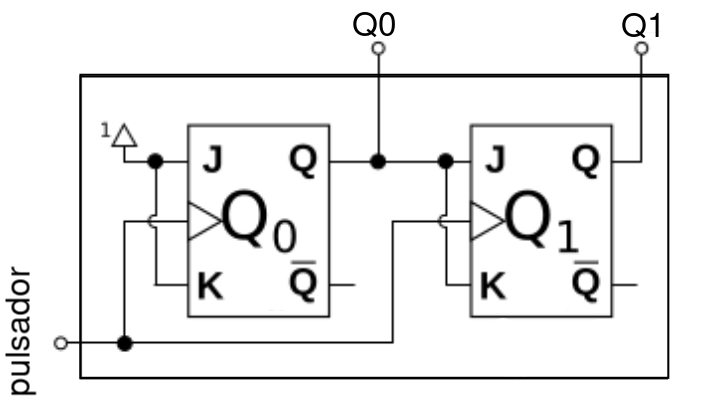
\includegraphics[scale=0.23]{circuito.png}
\end{figure}
\end{columns}
\begin{table}[h!]
\begin{tabular}{|c|c|c|c|c|}
\hline
Q$_1$(t) & Q$_0$(t) &  & Q$_1$(t+1) & Q$_0$(t+1) \\ \hline
0        & 0        &  & 0          & 1          \\ \hline
0        & 1        &  & 1          & 0          \\ \hline
1        & 0        &  & 1          & 1          \\ \hline
1        & 1        &  & 0          & 0          \\ \hline
\end{tabular}
\end{table}
Termine tabla de verdad, y ahora? A que se parece?$\to$ Un
contador!}




\end{frame}


\begin{frame}
\frametitle{Solución parte b}
  \only<1,2,3>{\begin{columns}
          \column{0.4\textwidth}
              Ya tenemos la tabla de verdad de este circuito, como lo usamos para lograr lo que queremos.
              Como empezamos...

            \pause
            \textbf{Tabla de verdad!}
          \column{0.5\textwidth}
          \pause
              \begin{figure}[h!]
                  \centering
                  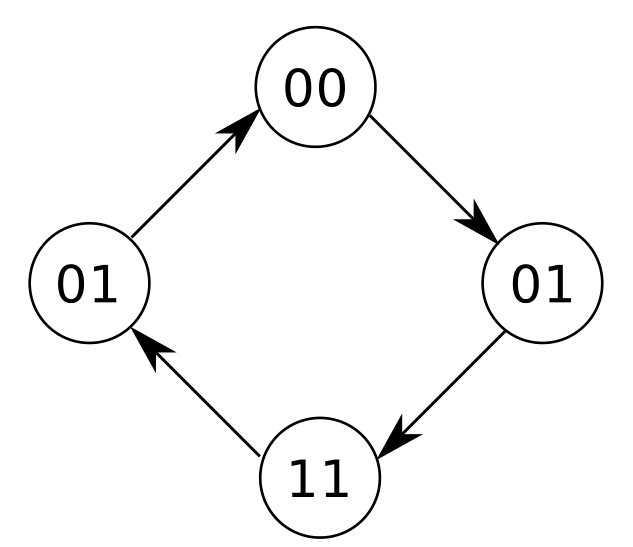
\includegraphics[scale=0.2]{ej1.png}
              \end{figure}
      \end{columns}
      \begin{table}[h!]
      \begin{tabular}{|c|c|c|c|c|}
      \hline
      Q$_1$(t) & Q$_0$(t) &  & Q$_1$(t+1) & Q$_0$(t+1) \\ \hline
      0        & 0        &  &           &          \\ \hline
      0        & 1        &  &           &           \\ \hline
      1        & 0        &  &           &           \\ \hline
      1        & 1        &  &           &           \\ \hline
      \end{tabular}
      \end{table}
      Vamos llenando
    }

      \only<4>{\begin{columns}
          \column{0.4\textwidth}
              Ya tenemos la tabla de verdad de este circuito, como lo usamos para lograr lo que queremos.
              Como empezamos...

            \textbf{Tabla de verdad!}
          \column{0.5\textwidth}
              \begin{figure}[h!]
                  \centering
                  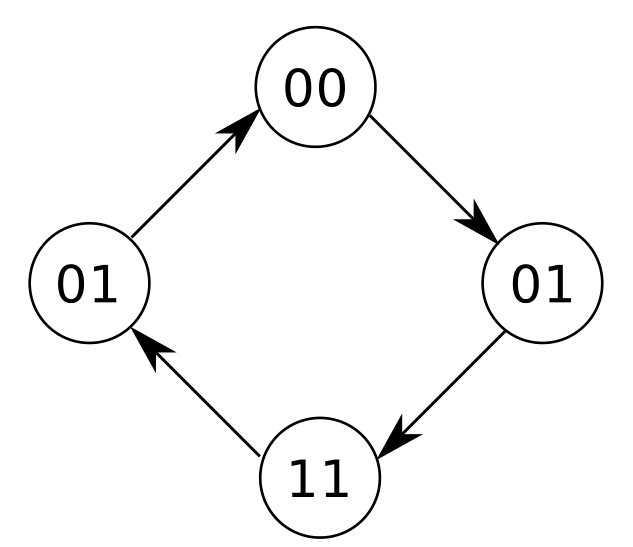
\includegraphics[scale=0.2]{ej1.png}
              \end{figure}
      \end{columns}
        \begin{table}[h!]
      \begin{tabular}{|c|c|c|c|c|}
      \hline
      Q$_1$(t) & Q$_0$(t) &  & Q$_1$(t+1) & Q$_0$(t+1) \\ \hline
      0        & 0        &  & 0          & 1          \\ \hline
      0        & 1        &  &           &           \\ \hline
      1        & 0        &  &           &           \\ \hline
      1        & 1        &  &           &           \\ \hline
      \end{tabular}
      \end{table}Tengo dos caminos...}
      \only<5>{
        \begin{columns}
          \column{0.4\textwidth}
              Ya tenemos la tabla de verdad de este circuito, como lo usamos para lograr lo que queremos.
              Como empezamos...

            \textbf{Tabla de verdad!}
          \column{0.5\textwidth}
              \begin{figure}[h!]
                  \centering
                  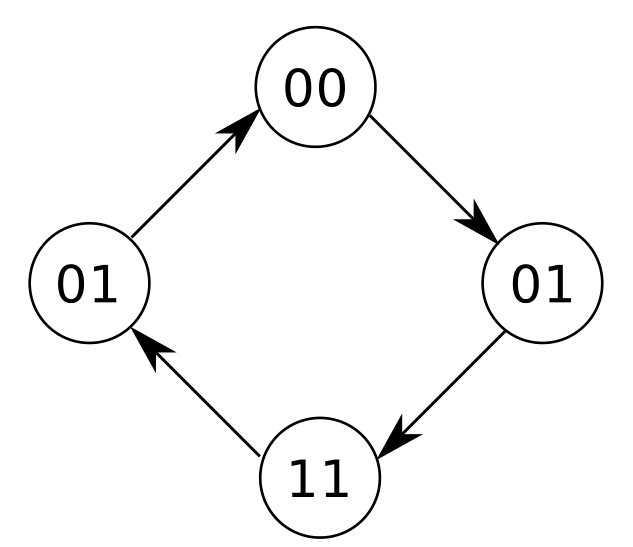
\includegraphics[scale=0.2]{ej1.png}
              \end{figure}
      \end{columns}
      \begin{table}[h!]
      \begin{tabular}{|c|c|c|c|c|}
      \hline
      Q$_1$(t) & Q$_0$(t) &  & Q$_1$(t+1) & Q$_0$(t+1) \\ \hline
      0        & 0        &  & 0          & 1          \\ \hline
      0        & 1        &  & ?          & ?          \\ \hline
      1        & 0        &  &           &           \\ \hline
      1        & 1        &  &           &           \\ \hline
      \end{tabular}
      \end{table}
    Lo dejo y sigo.}
      \only<6>{
        \begin{columns}
          \column{0.4\textwidth}
              Ya tenemos la tabla de verdad de este circuito, como lo usamos para lograr lo que queremos.
              Como empezamos...

            \textbf{Tabla de verdad!}
          \column{0.5\textwidth}
              \begin{figure}[h!]
                  \centering
                  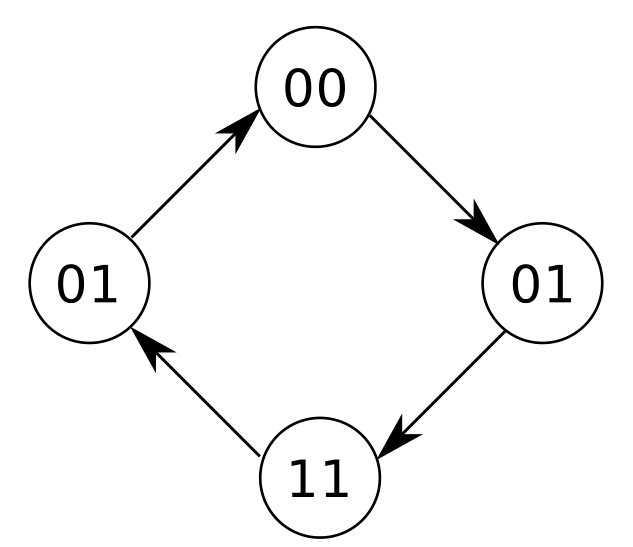
\includegraphics[scale=0.2]{ej1.png}
              \end{figure}
      \end{columns}
        \begin{table}[h!]
      \begin{tabular}{|c|c|c|c|c|}
      \hline
      Q$_1$(t) & Q$_0$(t) &  & Q$_1$(t+1) & Q$_0$(t+1) \\ \hline
      0        & 0        &  & 0          & 1          \\ \hline
      0        & 1        &  & ?          & ?          \\ \hline
      1        & 0        &  & -          & -          \\ \hline
      1        & 1        &  &           &           \\ \hline
      \end{tabular}
      \end{table}
    No me interesa este input.}
      \only<7>{\begin{columns}
          \column{0.4\textwidth}
              Ya tenemos la tabla de verdad de este circuito, como lo usamos para lograr lo que queremos.
              Como empezamos...

            \textbf{Tabla de verdad!}
          \column{0.5\textwidth}
              \begin{figure}[h!]
                  \centering
                  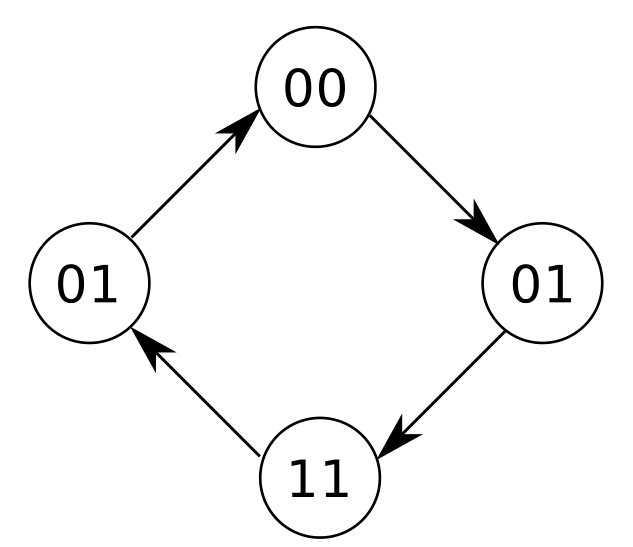
\includegraphics[scale=0.2]{ej1.png}
              \end{figure}
      \end{columns}
\begin{table}[h!]
      \begin{tabular}{|c|c|c|c|c|}
      \hline
      Q$_1$(t) & Q$_0$(t) &  & Q$_1$(t+1) & Q$_0$(t+1) \\ \hline
      0        & 0        &  & 0          & 1          \\ \hline
      0        & 1        &  & ?          & ?          \\ \hline
      1        & 0        &  & -          & -          \\ \hline
      1        & 1        &  & 0          & 1          \\ \hline
      \end{tabular}
      \end{table}Pero esto no parece funcionar.... Tengo indeterminación...}
\end{frame}


\begin{frame}
\frametitle{Solución parte b}

Parece que una misma entrada tiene que saber distinguir entre dos salidas distintas...
\pause
\vspace{0.5cm}

\begin{columns}
  \column{0.5\textwidth}
        \begin{figure}[h!]
            \centering
            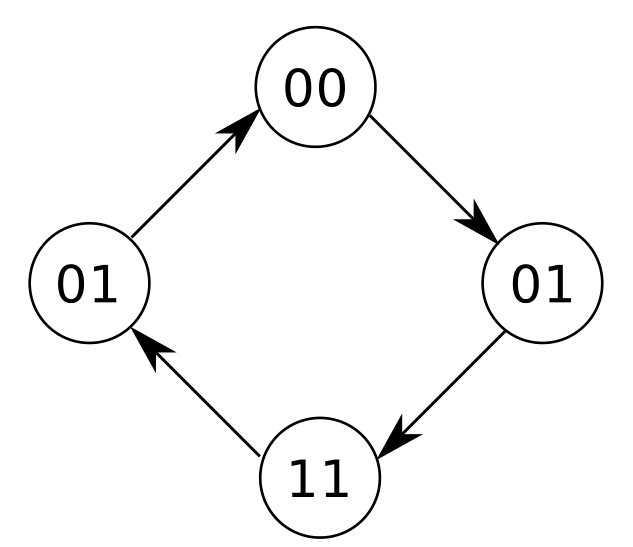
\includegraphics[scale=0.2]{ej1.png}
        \end{figure}
        \pause
    \column{0.5\textwidth}
     Pero gráficamente vemos que son dos estados diferentes.
   \vspace{0.3cm}
\pause

Primera idea, seria hacer alguna combinación de flip-flops para guardar el estado en el tiempo $t$ y
en el tiempo $t-1$, y ver de salvar en el caso $t=0$...
   \vspace{0.3cm}
\pause

Otra forma m\'as inteligente, sería renombrar los estados del sumador (por algo nos dieron ese circuito...)

\end{columns}
\end{frame}

\begin{frame}
  \frametitle{Solución parte b}
\begin{table}[h!]
\begin{tabular}{|c|c|c|c|c|}
\hline
Q$_1$ & Q$_0$ & $\to$ & o$_1$ & o$_0$ \\ \hline
0        & 0        & $\to$ & 0          & 0          \\ \hline
0        & 1        &$\to$  & 0          & 1          \\ \hline
1        & 0        &$\to$  & 1          & 1          \\ \hline
1        & 1        &$\to$  & 0          & 1          \\ \hline
\end{tabular}
\end{table}

\pause
Y esto como lo implemento?
\pause

Por ahora tenemos el pulsador al circuito dado (contador) y la salida de este
queremos transformarlo a lo pedido. Y como encuentro el circuito?

\pause
Suma de producto y producto de suma!
\end{frame}

\begin{frame}
\frametitle{Solución parte b}
\begin{columns}
    \column{0.5\textwidth}
        \begin{table}[h!]
            \begin{tabular}{|c|c|c|c|c|}
            \hline
            Q$_1$ & Q$_0$ & $\to$ & o$_1$ & o$_0$ \\ \hline
            0        & 0        & $\to$ & 0          & 0          \\ \hline
            0        & 1        &$\to$  & 0          & 1          \\ \hline
            1        & 0        &$\to$  & 1          & 1          \\ \hline
            1        & 1        &$\to$  & 0          & 1          \\ \hline
            \end{tabular}
            \end{table}

    \column{0.5\textwidth}
    \pause
    $o_1$ tiene un único 1 $\to$ suma de productos.
    \pause

    Que producto de $Q_1=1$ con $Q_0=0$ me da 1?
    \pause

    $o_1$ = Q$_1$ * $\overline{\text{Q}_0}$  \pause $\to$ OR
    \vspace{1cm}
    \pause

    $o_0$ tiene un único 0 $\to$ producto de sumas.
\pause

  Que suma de $Q_1=0$ con $Q_0=0$ me da 0?
\pause

    $o_0$ = Q$_1$ + Q$_0$ \pause $\to$ AND con  Q$_0$ negada

\end{columns}
\end{frame}

\begin{frame}
\frametitle{Solución parte b}

Nos quedaría:
\begin{figure}[h!]
    \centering
    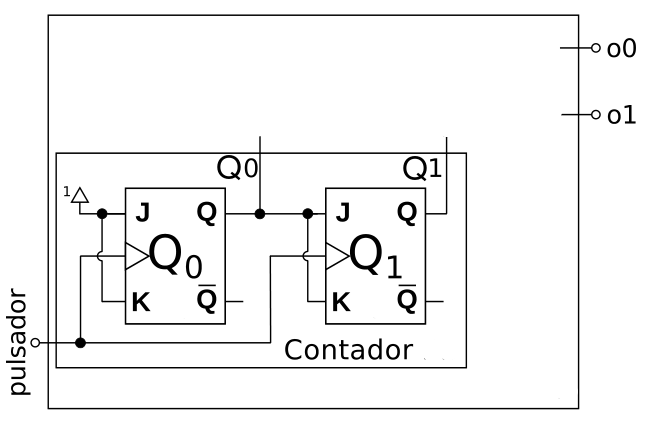
\includegraphics[scale=0.3]{circuito0.png}
\end{figure}
\end{frame}
\begin{frame}
\frametitle{Conclusion}
\begin{itemize}
  \item Funcionamiento de Flip-Flop JK.\pause
  \item Implementación para crear un contador.\pause
  \item Noción de estados.\pause
  \item Renombrar con bloque combinacional.
\end{itemize}

\end{frame}
\end{document}
